% 例 1 折线问题：AB∥CD，过 P 作 PE∥AB，∠APC = ∠BAP + ∠DCP
\documentclass[tikz,border=4pt]{standalone}
\usepackage{ctex}
\usepackage{amsmath}
\usetikzlibrary{calc, arrows.meta, decorations.markings}
\begin{document}
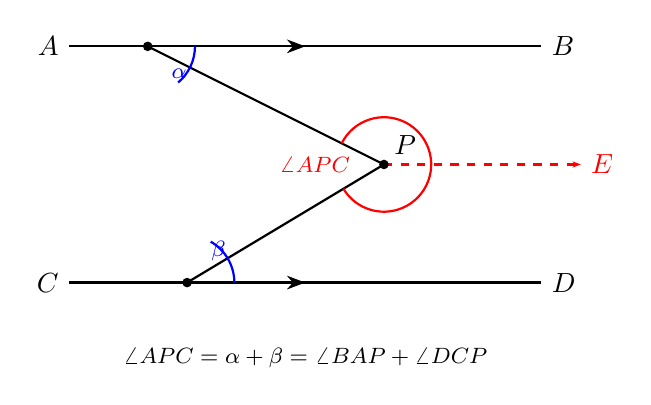
\begin{tikzpicture}[scale=1.0, thick,
  arrowone/.style={postaction={decorate, decoration={markings,
    mark=at position 0.5 with {\arrow{Stealth}}}}}]
  % AB 上方水平，CD 下方水平
  \draw[arrowone] (0,3) -- (6,3);
  \node[left] at (0,3) {$A$}; \node[right] at (6,3) {$B$};
  \draw[arrowone] (0,0) -- (6,0);
  \node[left] at (0,0) {$C$}; \node[right] at (6,0) {$D$};
  % P 在中间
  \coordinate (A) at (1,3);
  \coordinate (C) at (1.5,0);
  \coordinate (P) at (4,1.5);
  \draw (A) -- (P) -- (C);
  % 辅助线 PE 平行 AB（红虚线，向右延伸）
  \draw[red, dashed, -{Stealth[length=3pt]}] (P) -- (6.5,1.5);
  \node[red, right] at (6.5,1.5) {$E$};
  % 标角
  \draw[blue] ($(A)+(0.6,0)$) arc (0:-50:0.6);
  \node[blue, font=\footnotesize] at ($(A)+(0.4,-0.35)$) {$\alpha$};
  \draw[blue] ($(C)+(0.6,0)$) arc (0:60:0.6);
  \node[blue, font=\footnotesize] at ($(C)+(0.4,0.4)$) {$\beta$};
  % ∠APC 总角
  \pgfmathsetmacro{\angAP}{atan2(3-1.5, 1-4)} % 朝 A
  \pgfmathsetmacro{\angCP}{atan2(0-1.5, 1.5-4)} % 朝 C
  \draw[red, thick] ($(P)+({0.6*cos(\angAP)},{0.6*sin(\angAP)})$) arc (\angAP:\angCP:0.6);
  \node[red, left, font=\footnotesize] at ($(P)+(-0.3,0)$) {$\angle APC$};
  \filldraw (A) circle (1.3pt);
  \filldraw (C) circle (1.3pt);
  \filldraw (P) circle (1.3pt) node[above right] {$P$};
  \node[below, font=\footnotesize] at (3,-0.7) {$\angle APC = \alpha + \beta = \angle BAP + \angle DCP$};
\end{tikzpicture}
\end{document}
